% Paper compiled from RevTeX 4.2 Template (Overleaf)

\documentclass[preprint,
letterpaper,
 amsmath,amssymb,
 aps,
%floatfix,
]{revtex4-2}

\usepackage{graphicx}% Include figure files
\usepackage{dcolumn}% Align table columns on decimal point
\usepackage{bm}% bold math
\usepackage{hyperref}% add hypertext capabilities
\usepackage[mathlines]{lineno}% Enable numbering of text and display math
\usepackage{setspace}
\usepackage{siunitx}
\usepackage{enumitem}
\newcommand{\ts}{\textsuperscript}
\usepackage{amsmath}

\usepackage[utf8]{inputenc}
\usepackage{float}
\newcommand{\iu}{{i\mkern1mu}}
\def\code#1{\texttt{#1}}

\doublespacing
\begin{document}

\title{Gravitational Wave Detection:\\
Event GW170814 and the performance of matched filtering and $\chi^2$-consistency testing in the presence of Gaussian noise, non-Gaussianly distributed noise, and transient glitches}
\author{Vinh Nguyen}
\email[Mentored by Dr. Eric Myers – Department of Physics and Astronomy, State University of New York at New Paltz]{}
\affiliation{Klein Oak High School, Spring, TX 77379}
\date{July 29, 2020}
\begin{abstract}
The detection of gravitational wave signals of astrophysical origins is particularly challenging because the signals are always contaminated by noise. Two of most prominent and efficient detection techniques currently used in Virgo/LIGO search pipelines are matched filtering and $\chi^2$-consistency testing. This paper investigated the performance of these two detection techniques in event GW170814 as well as in the presence of both consistently distributed noise and transient glitches. It was found that matched filtering performs best in the presence of perfect or close-perfect Gaussian noise; it can also mistake glitches for real gravitational waves if certain types of glitches are present. Additionally, it was found that $\chi^2$-consistency testing has little effects in cases where matched filtering had previously been unsuccessful. Finally, it was shown that the use of $\chi^2$-consistency testing is crucial to detecting and identifying gravitational waves in the presence of \textit{Extremely Loud} and \textit{Blip} glitches.
\end{abstract}

\maketitle
\section{Introduction}
The existence of gravitational waves was first predicted by Albert Einstein in 1916 as a direct result of his Theory of General Relativity. Since then, gravitational wave science and detection have been a leading scientific field of interest for not just physicists, but also astronomers, geologists, material scientists, and engineers as well. With the first confirmed detection of gravitational waves from a binary black hole merger in 2015 (event GW150914), the prospects of gravitational wave science and its applications to other fields have only become brighter. As of July 2020, there exists four primary fully functioning gravitational wave detectors – the LIGO Hanford Detector in Washington, the LIGO Livingston Detector in Louisiana, the Virgo Observatory in Italy, and the KAGRA detector in Japan. 

The detection of gravitational waves, however, poses many challenges, for their signals are extremely weak. Gravitational wave signals can be easily contaminated by noise, thereby requiring a wide range of sophisticated mathematical and data analysis techniques to be identified. This paper explores several complications in the detection of gravitational waves – specifically, it studies the detection of event GW170814 as well as the general performance of matched filtering and $\chi^2$-consistency testing in different unfavorable noise conditions present in the Virgo and LIGO gravitational wave detectors.

This paper uses real Virgo/LIGO data queried from the Gravitational Wave Open Science Center (GWOSC). GWOSC is a collaborative effort between the LIGO Laboratory, the LIGO Scientific Collaboration and the Virgo Collaboration to provide the public with gravitational wave data from the two LIGO facilities (Hanford, WA and Livingston, LA) as well the Virgo Observatory in Cascina, Italy. The structure of this paper is as follows. \textit{Section \ref{background}} provides detailed background information necessary for the methods undertaken in this paper. Specifically, \textit{sub-section \ref{gw and ligo}} discusses gravitational waves, its detection and current detector technology while \textit{sub-section \ref{data anal}} addresses data analysis details such as  the Fourier transform, noise characteristics, matched filtering and $\chi^2$-consistency testing. \textit{Section \ref{method}} gives a detailed description of this paper's methodology and the steps undertaken. \textit{Section \ref{results}} provides the paper's preliminary results in addition to data analysis. \textit{Section \ref{conclusions}} presents the study's conclusions and proposals for possible future research directions. Finally, \textit{section \ref{summary}} gives a brief overall summary of this paper's content. 

\section{Background} \label{background}
\subsection{Gravitational waves and the Laser Interferometer Gravitational-Wave Observatory (LIGO)} \label{gw and ligo}
In 1915, Albert Einstein first published his theory of general relativity, describing space and time as one four-dimensional concept called \textit{``space-time''} \cite{maggiore_2008}, In this theory, he describes the force of gravity not as an inherent property that a massive body possesses, but rather as a byproduct of curved space-time. To put this more simply, we can say that a body with mass warps space-time, thereby creating a gravitational field surrounding it, affecting other bodies \cite{carlip}. To understand this idea, we can make use of an analogy: suppose that the fabric of space-time is a rubber sheet, and that any object with mass on it warps the surrounding area (FIG. 1.), hence creating a gravitational field. It follows from Einstein's Theory of Relativity that rapid changes in the curvature of space-time would produce ripples, called \textit{gravitational waves} (abbreviated as GW), that propagate outward at the speed of light  \cite{JSTORLIGO}.

\begin{figure}[t]
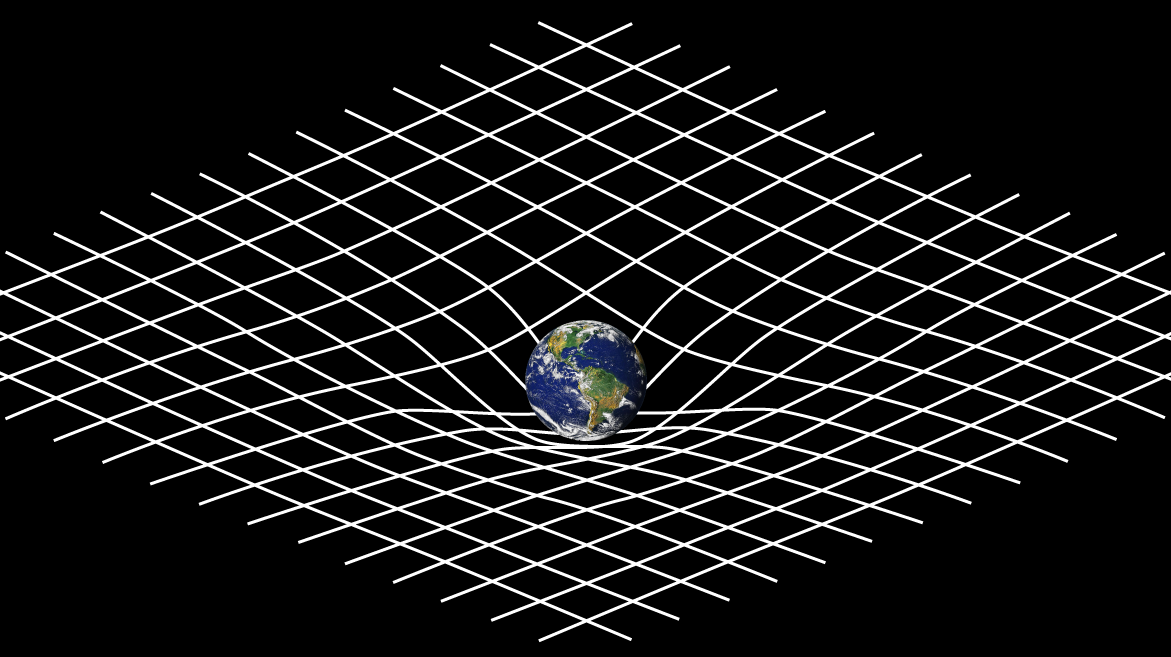
\includegraphics[width=8cm]{genral.png}
\caption{This figure shows a simplified analogy for Einstein's idea of space-time – which cannot be fully illustrated by a 2D picture. Adapted from \cite{mattson}.}
\centering
\end{figure}

LIGO (short for Laser Interferometer Gravitational-wave Observatory) is an NSF-funded, large scale scientific collaboration between the California Institute of Technology and the Massachusetts Institute of Technology designed to detect gravitational waves. As of June 2020, LIGO has two site locations – one in Hanford, Washington and the other in Livingston, Louisiana. Another important scientific collaboration is the Virgo project. The Virgo project is a European collaboration for gravitational wave detection funded by the French Centre National de Recherche Scientifique (CNRS), the Italian Istituto Nazionale della Fisica Nucleare (INFN), the Dutch Nikhef in addition to the Polish and Hungarian institutes \cite{collaboration2019open}. Virgo has one detector located in Cascina, Italy. The two LIGO sites as well as the Virgo site in Italy each employs a type of detector called the Michelson Fabry-Perot Interferometer (interferometer for short) \cite{creighton_anderson_2011}. Virgo/LIGO's interferometers function by using four test masses (in this case, mirrors) in an L-shaped configuration, hung by wires near the ends and the vertex of the `L' as shown in FIG. 2. The test masses are configured so that the length $L_1 \approx L_2 = L$ (note that at the frequency of around $1$ Hz, the test masses can move freely horizontally) \cite{JSTORLIGO}. 

\begin{figure}
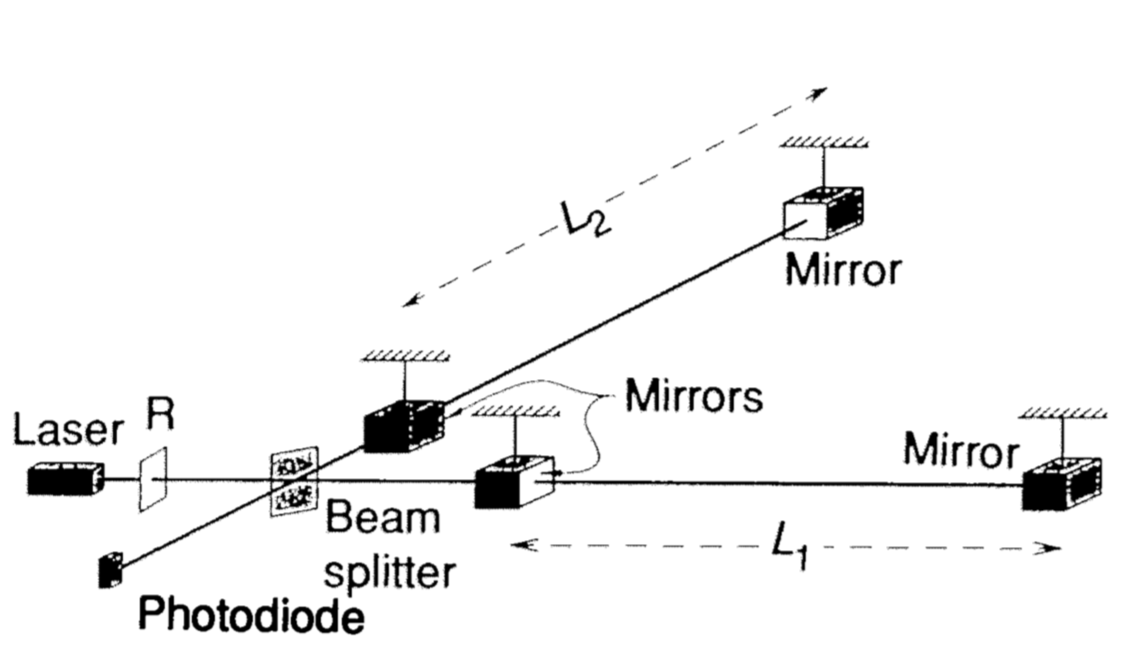
\includegraphics[width = .6\textwidth]{Interferometer.png}
\caption{A simplified diagram of the Michelson Fabry-Perot Interferometer. Adapted from \cite{JSTORLIGO}.}
\centering
\end{figure} 
\begin{figure}[!tbp]
  \centering
  \begin{minipage}[b]{0.48\textwidth}
    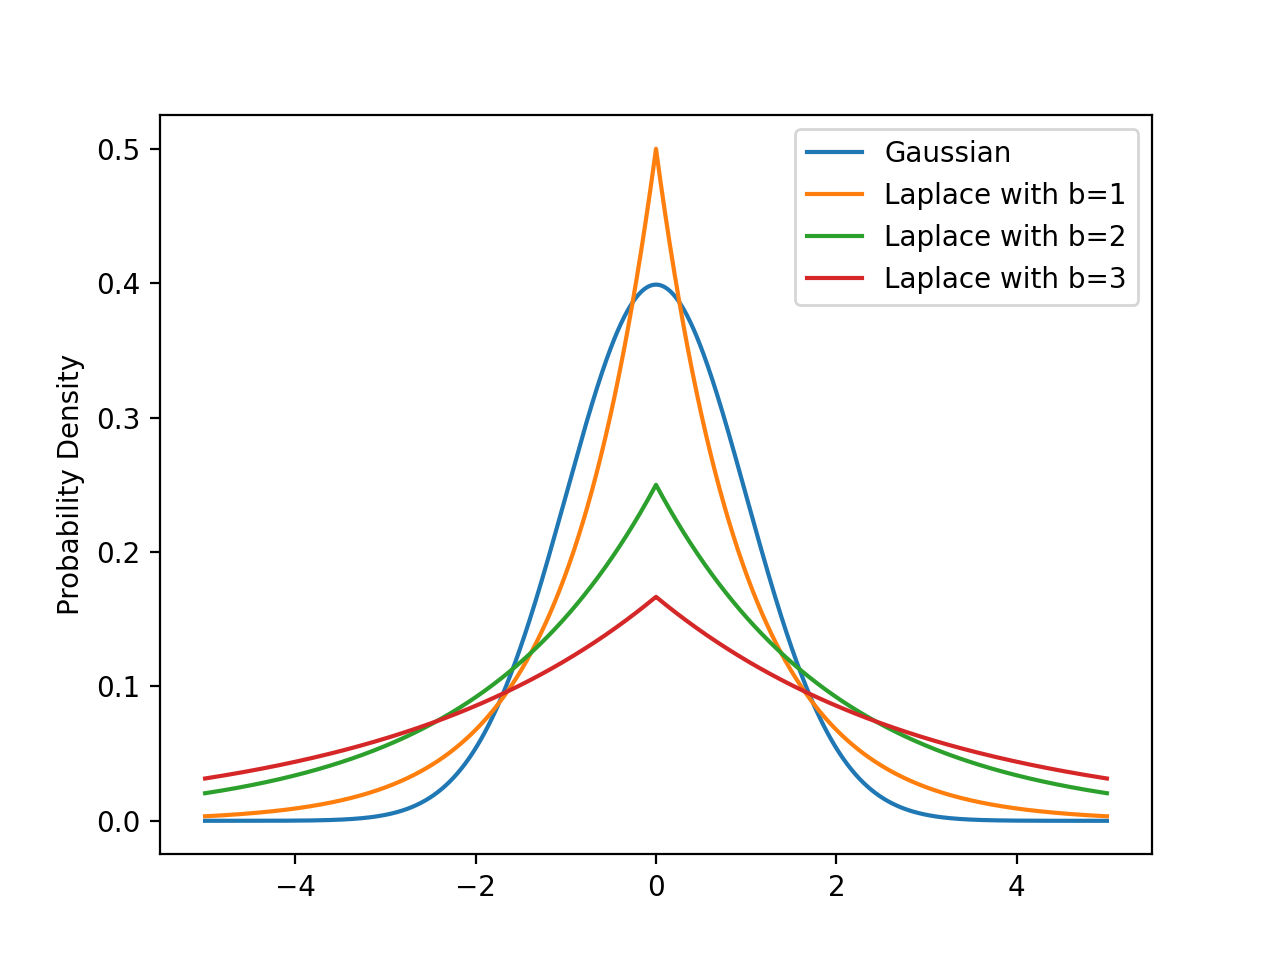
\includegraphics[width = \textwidth]{pdf graphs.png}
    \caption{The different probability density functions $f_X(x)$ are shown. Since $\int_{-\infty}^\infty f_X(x)dx = 1$, the lower the  functions' maximums are, the heavier their tails must be, leading to higher kurtoses.}
  \end{minipage}
  \hfill
  \begin{minipage}[b]{0.48\textwidth}
    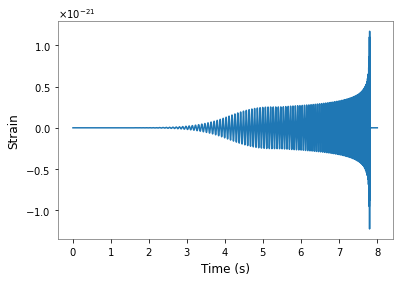
\includegraphics[width = \textwidth]{template.png}
    \caption{This figure shows the template waveform strain time-series of a binary black hole merger with masses 30 $M$\textsubscript{\(\odot\)} and 23 $M$\textsubscript{\(\odot\)} generated with PyCBC \cite{pycbc}.}
  \end{minipage}
\end{figure}
If there is a gravitational wave passing in between the test masses, the space between them will be stretched and compressed, squeezing one arm while stretching the other such that we can calculate the value of the arm length difference $\Delta L = L_1 - L_2$ \cite{teacherintro}. To measure this quantity $\Delta L$, the device uses a technique called laser interferometry \cite{LIGOArxiv}. Specifically, a powerful laser beam is shined at the beam splitter, thereby splitting the beam in half along the two arms. These beams then each enter a Fabry-Perot cavity where they are reflected back and forth between the mirrors, building up the laser light within the interferometer and increasing the distance travelled by the beam \cite{fabry} – thereby increasing the interferometer's sensitivity. As the laser beams in the two arms exit the Fabry-Perot cavity and return to the beam splitter, the splitter recombines the two half-beams and gives off a portion of the combined beam to a photodiode – hence allowing scientists to analyze the interference patterns of the waves using optics principles, and thus determine the quantity $\Delta L$. 

For gravitational waves passing through the test masses, the fractional difference in arm length $\frac{\Delta L}{L}$ is the strain $h$ (a quantity that measure the `strength' of gravitational waves) of the waves. Mathematically, the strain $h(t) = \frac{\Delta L(t)}{L}$ can also be expressed as a linear combination of its cross and plus polarizations, as follows \cite{JSTORLIGO}:
\begin{equation}
h(t) = F_\times h_\times (t) + F_+ h_+ (t)
\end{equation}

\subsection{LIGO Data Analysis and Conventions} \label{data anal}
\subsubsection{The Fourier Transform}
The signal from Virgo/LIGO is recorded as a function of time. However, to process this signal, we must usually transform the signal from its original time-domain into its frequency-domain through the use of a mathematical tool called the \textit{Fourier Transform}. In simplest terms, the Fourier Transform decomposes a function into its frequency content. Given a \textit{continuous} time-series function $F(t)$, its frequency-domain representation $\widetilde{F}(f)$ is given by \cite{dsptextbook}:
\begin{equation}
\widetilde{F}(f) = \int_{-\infty}^{\infty}F(t)e^{-2\pi\iu ft} dt
\end{equation}

Notice that $\widetilde{F}(f)$ is a complex-valued function whose magnitude represents the frequency amplitude and whose argument represents the phase offset. Similarly, a frequency-domain continuous function $\widetilde{F}(f)$ can also be transformed back into its time-domain representation using an \textit{inverse Fourier Transform}. Given $\widetilde{F}(f)$, $F(t)$ can be calculated by the equation:
\begin{equation}
F(t) = \int_{-\infty}^{\infty}\widetilde{F}(f)e^{2\pi\iu ft} df
\end{equation}

Unfortunately, LIGO signal is not a continuous function in the time-domain, thus we have to \textit{discretize} our formulas for both the continuous forward and the continuous inverse Fourier Transforms \cite{dsptextbook}. Given a time-domain signal \textit{sequence} $f[n]$, the frequency-domain representation $\widetilde{f}[n]$ can be obtained using the Discrete Fourier Transform (DFT) as follows\cite{roberts_2020}:
\begin{equation}
\widetilde{f}[n]=\sum _{n=0}^{N-1}f[n]\cdot e^{-{\frac {2\pi}{N}\iu kn}}
\end{equation}

The time-domain sequence $f[n]$ can be then obtained from the frequency-domain sequence $\widetilde{f}[n]$ through the inverse discrete Fourier transform (with a normalization factor) as such \cite{roberts_2020}:
\begin{equation}
f[n]=\frac{1}{N}\sum _{n=0}^{N-1}\widetilde{f}[n]\cdot e^{{\frac {2\pi}{N}\iu kn}}
\end{equation}

Since we are working with discrete-valued sequences, performing a DFT would give rise to what we call \textit{spectral leakages}. When the Fourier Transform is applied onto a finite, non-periodic data segment (i.e.\ Virgo/LIGO data), false frequency amplitudes might occur. The reason for this is that since the transformation is discrete in nature, frequencies that lies in between or across multiple frequency intervals can falsely create high amplitudes. Thus, to minimize this, we always apply a windowing function to data – tapering the data segment's ends, making it periodic – whenever the use of the DFT is required (note that windowing does not decrease spectral leakage, but rather re-distributes the leakage effect so that it causes the least harm). In this paper, I used a computer algorithm that implements the Discrete Fourier Transform called the Fast Fourier Transform (FFT) which is included within the Python PyCBC library \cite{numpy}.

\begin{figure}[!tbp]
  \centering
  \begin{minipage}[b]{0.48\textwidth}
    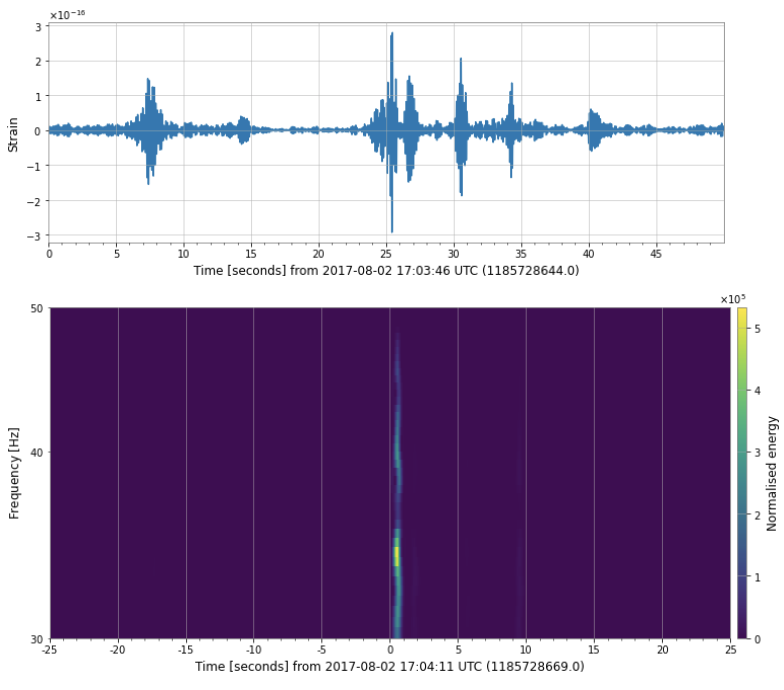
\includegraphics[width=\textwidth]{loud 69 graphics.png}
    \caption{The top figure shows the strain time-series of 50 seconds around Glitch 1. The bottom figure shows a Q-transformed spectrogram around Glitch 1. (Data queried from \cite{collaboration2019open})}

  \end{minipage}
  \hfill
  \begin{minipage}[b]{0.48\textwidth}
    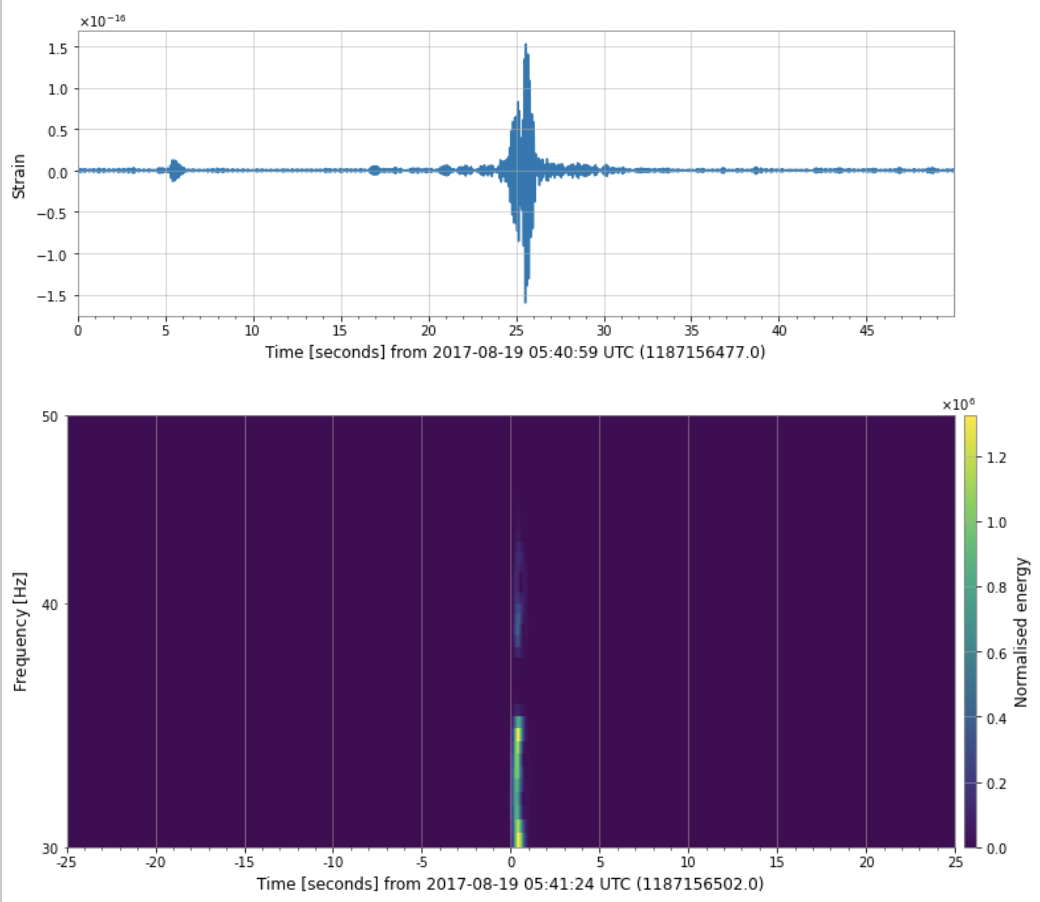
\includegraphics[width=\textwidth]{loud 02 graphics.png}
    \caption{The top figure shows the strain time-series of 50 seconds around Glitch 2. The bottom figure shows a Q-transformed spectrogram around Glitch 2. (Data queried from \cite{collaboration2019open})}
  \end{minipage}
\end{figure}


 \begin{figure}[!tbp]
  \centering
  \begin{minipage}[b]{0.48\textwidth}
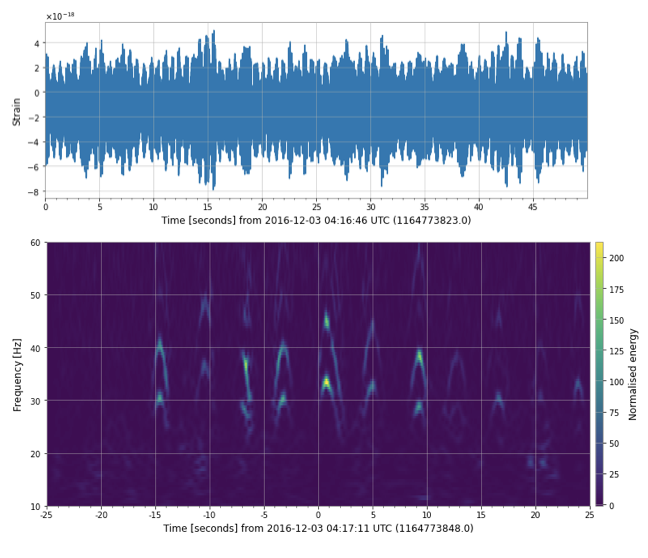
\includegraphics[width=\textwidth]{Scattered Light Graphics.png}
\caption{The top figure shows the strain time-series of 50 seconds around Glitch 3. The bottom figure shows a Q-transformed spectrogram around Glitch 3. (Data queried from \cite{collaboration2019open})}
  \end{minipage}
  \hfill
  \begin{minipage}[b]{0.48\textwidth}
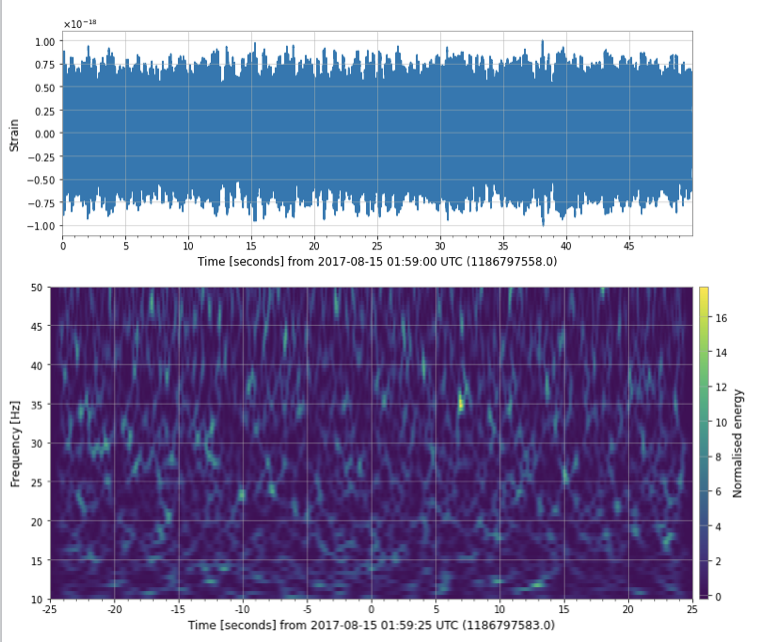
\includegraphics[width=\textwidth]{power line graphics.png}
\caption{The top figure shows the strain time-series of 50 seconds around Glitch 4. The bottom figure shows a Q-transformed spectrogram around Glitch 4. (Data queried from \cite{collaboration2019open})}
  \end{minipage}
\end{figure}

 \begin{figure}[!tbp]
  \centering
  \begin{minipage}[b]{0.48\textwidth}
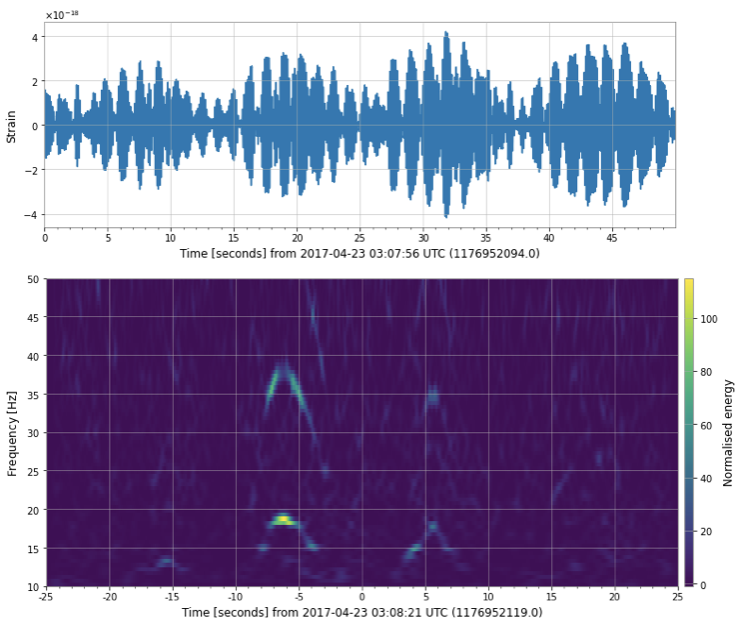
\includegraphics[width=\textwidth]{whistle graphics.png}
\caption{The top figure shows the strain time-series of 50 seconds around Glitch 5. The bottom figure shows a Q-transformed spectrogram around Glitch 5. (Data queried from \cite{collaboration2019open})}
  \end{minipage}
  \hfill
  \begin{minipage}[b]{0.48\textwidth}
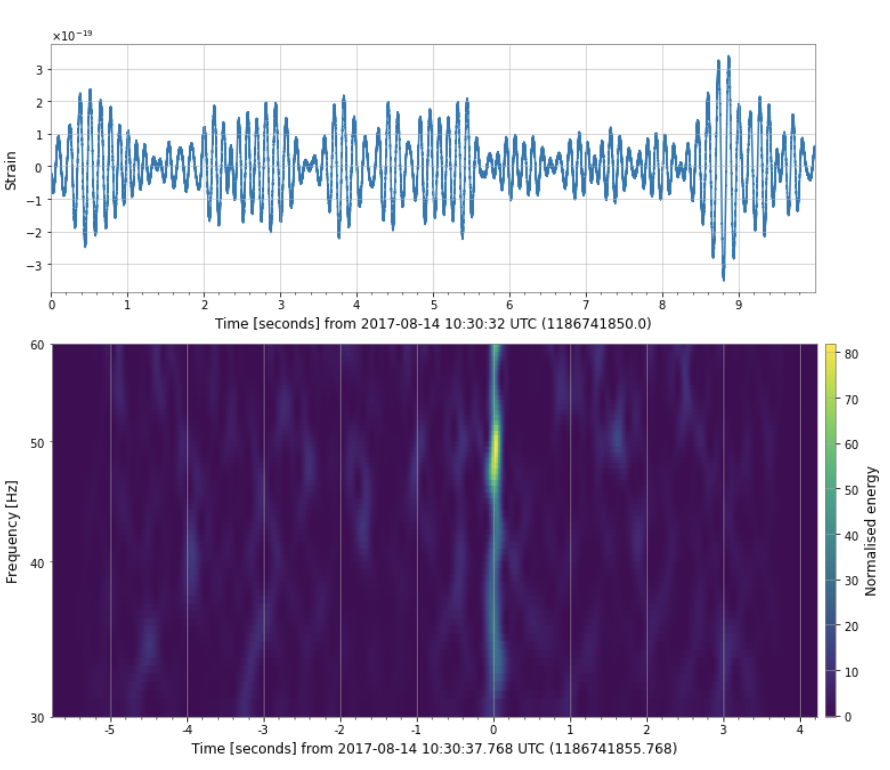
\includegraphics[width=\textwidth]{blipppppp.png}
\caption{The top figure shows the strain time-series of 10 seconds around the Blip glitch near event GW170814 found at LIGO Livingston. The bottom figure shows a Q-transformed spectrogram around the same glitch. \cite{collaboration2019open}}
  \end{minipage}
\end{figure}

\subsubsection{Noise characteristics}
Being able to reach a strain sensitivity of $10^{-23}/\sqrt{\text{Hz}}$ \cite{sensitivity} means Virgo/LIGO's interferometers are extremely sensitive to any changes in the arm lengths – which can be caused by distorted space-time due to gravitational waves, or by vibrations that move the test masses. Thus, recorded signal $s(t)$ includes not only gravitational waves, but also unwanted vibrations from other sources as well \cite{ultimate}. Any unwanted noise, even on the smallest of scales, can still significantly interfere with data recorded by Virgo/LIGO's interferometers. Virgo/LIGO noise comes from many sources, but some examples include seismic noise due to motions of the Earth's surface, thermal noise at the molecular level affecting the test masses, and quantum shot noise at high frequencies caused by the quantum nature of light \cite{blair_howell_ju_zhao_2012}.


In order to extract buried gravitational wave signals from noise, we must first understand the statistical properties of the noise. Noise is said to be stationary if its statistical properties do not significantly change over time. Another important noise characteristic is its Gaussianity. Given \textit{`Gaussian'} noise with a time-series function $n(t)$, both the real and imaginary components of its Fourier Transform $\widetilde{n}(f)$ follow the normal distribution \cite{yamamoto}; that is, $\Re[\widetilde{n}(f)]$ and  $\Im{[\widetilde{n}(f)]}$ have a probability density function (PDF) of:
\begin{equation}
    p(x) = \frac{1}{\sigma\sqrt{2\pi}}\exp{\left(-\frac{1}{2}\frac{(x-\mu)^2}{\sigma^2}\right)}
\end{equation}
where $\sigma^2$ is the sample variance and the mean $\mu = 0$. By the Central Limit Theorem in statistics, a set of random noise sample naturally tends to the Gaussian distribution if sufficiently large data samples were taken \cite{jaranowski2007gravitationalwave}. Nonetheless, real Virgo/LIGO noise can still deviate from this theoretical normality. Aside from the Gaussian distribution, noise can also follow a variety of different probability density distributions such as the Poisson distribution or the Laplace distribution. Although it is not common in real-life Virgo/LIGO operations that these noise models are present, this paper still considers the case of Laplacian noise for theoretical analysis purposes. Furthermore, there also exists abrupt, transient noise sources of, sometimes, unknown origins called glitches \cite{ultimate}. Glitches can be grouped into a variety of classifications according Gravity Spy's \textit{`Field Guide'} \cite{gravityspy}. In this paper, we only primarily discuss five types of glitches: \textit{Extremely Loud}, \textit{Scattered Light}, \textit{Power Line}, \textit{Whistle}, and \textit{Blip}. \textit{Extremely Loud} is a broad classification for major detector disturbances such as photodiode saturation, causing loud and high energy transient noise bursts. \textit{Scattered Light} glitches are caused by malfunctions in the optical mechanisms of Virgo/LIGO; they look like upward humps and are particularly harmful in searching for binary inspirals \cite{gravityspy}. The third classification of glitches is called \textit{Power Line}; \textit{Power Line} glitches are caused by electrical equipments such as air compressors that use alternating current (AC). The fourth classification is called \textit{Whistle} glitches; they are usually reverse V-shaped and are caused by radio signals \cite{gravityspy}. Finally, \textit{Blip} glitches are very short duration ($\approx 40$ms) noise bursts at frequencies between 30 and 500 Hz. As of currently, there are no known causes and thus \textit{Blip} glitches are the most damaging to the detection of gravitational waves \cite{gravityspy}. It is worth pointing out that over short time intervals, though, Virgo/LIGO noise can still be reasonably approximated to be Gaussian and stationary \cite{collaboration2019open}.

\begin{widetext}
\begin{figure}[t]
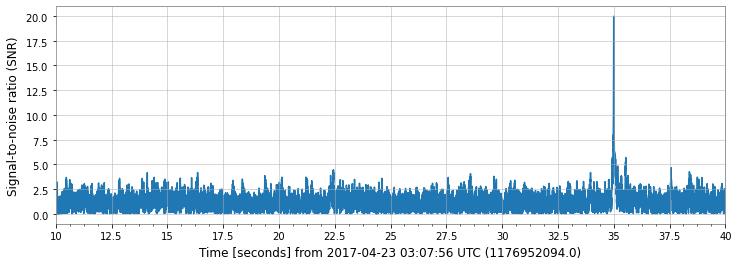
\includegraphics[width = .9\textwidth]{gaussian -21 template 1.png}
\caption{This figure shows the resulting cropped SNR $\rho(t)$ after matched filtering was applied to recover the template signal from perfectly Gaussian noise scaled down by a factor of $10^{-21}$. A signal peak was detected at time $t = 35.0$s with SNR $\rho = 20.0$}
\centering
\end{figure} 

\begin{figure}[t]
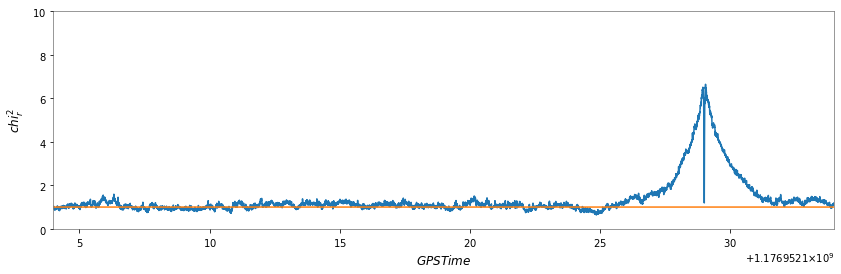
\includegraphics[width = .9\textwidth]{chi2 gaussian zoomed.png}
\caption{This figure shows the resulting $\chi^2_r$ statistic for perfectly Gaussian noise scaled down by a factor of $10^{-21}$. A strong dip toward unity is clearly seen at the expected time $t=35s$.}
\centering
\end{figure} 

\begin{figure}[t]
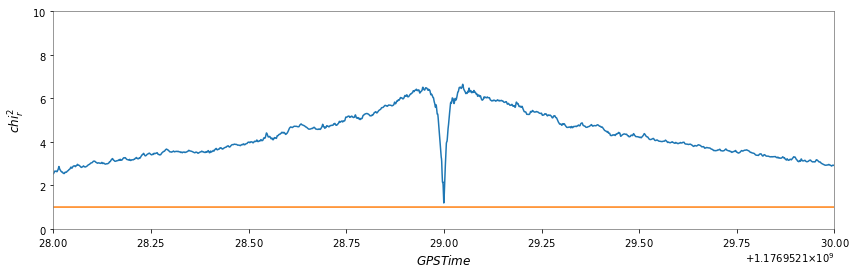
\includegraphics[width = .9\textwidth]{chi2 gaussian.png}
\caption{This figure shows the resulting $\chi^2_r$ statistic for perfectly Gaussian noise scaled down by a factor of $10^{-21}$, zoomed in to just the two-second interval between the time of expected signal.}
\centering
\end{figure} 

\begin{figure}[t]
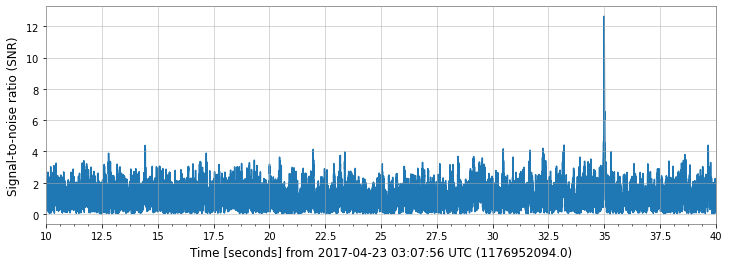
\includegraphics[width = .9\textwidth]{laplacian b=1 template 1.png}
\caption{This figure shows the resulting cropped SNR $\rho(t)$ after matched filtering was applied to recover the template signal from perfectly Laplacian noise with $b=1$, scaled down by a factor of $10^{-21}$. A signal peak was detected at time $t = 35.0$s with SNR $\rho = 12.6$.}

\centering
\end{figure} 

\begin{figure}[t]
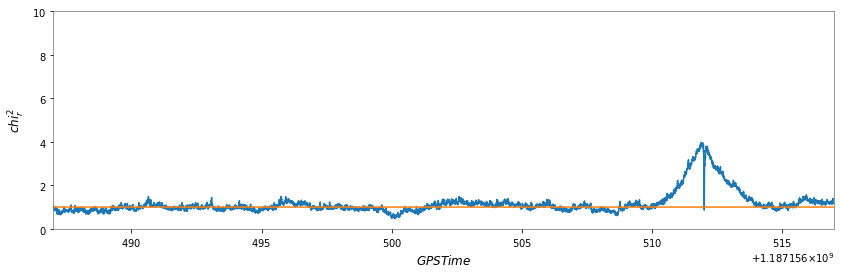
\includegraphics[width = .9\textwidth]{chi2 laplace b=1 zoomed.png}
\caption{This figure shows the resulting $\chi^2_r$ statistic for perfectly Laplacian noise with $b=1$ scaled down by a factor of $10^{-21}$. A strong dip toward unity is seen at time $t = 35.0$s with climbing values just around it.}
\centering
\end{figure} 
\end{widetext}

\begin{widetext}

\begin{figure}[t]
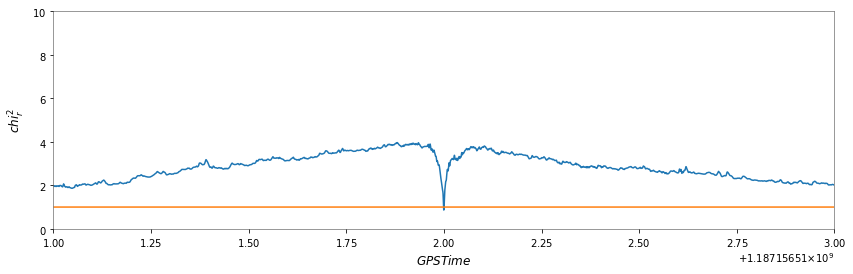
\includegraphics[width = .9\textwidth]{chi2 laplace b=1.png}
\caption{This figure shows the resulting $\chi^2_r$ statistic for perfectly Laplacian noise with $b=1$ scaled down by a factor of $10^{-21}$. The graph is zoomed in to show just the two-second time interview around the time of expected signal. A strong dip toward unity is seen at time $t = 35.0$s.}
\centering
\end{figure} 


\begin{figure}[t]
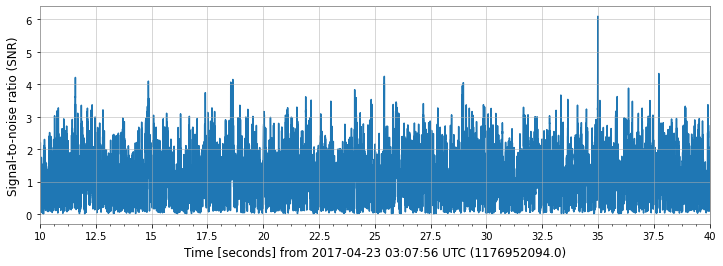
\includegraphics[width = .9\textwidth]{laplacian b=2 template 1.png}
\caption{This figure shows the resulting cropped SNR $\rho(t)$ after matched filtering was applied to recover the template signal from perfectly Laplacian noise with $b=2$, scaled down by a factor of $10^{-21}$. A signal peak was detected at time $t = 35.0$s with SNR $\rho = 6.1$.}
\centering
\end{figure} 

\begin{figure}[t]
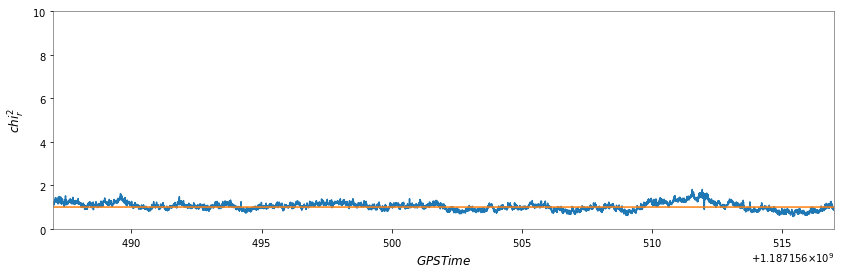
\includegraphics[width = .9\textwidth]{chi2 laplace b=2 zoomed.png}
\caption{This figure shows the resulting $\chi^2_r$ statistic for perfectly Laplacian noise with $b=2$ scaled down by a factor of $10^{-21}$. A small dip toward unity is seen at time $t = 35.0$s.}
\centering
\end{figure} 
\end{widetext}
\subsubsection{Matched filtering}
The primary goal of Virgo/LIGO data analysis is to determine if there is gravitational wave signal buried in the noise. There are many ways that this can be accomplished; however, the most efficient and effective method is called \textit{matched filtering}, especially in cases where noise is both Gaussian and stationary \cite{helstrom_1975}. Matched filtering allows the recorded data stream to be searched for the presence of a known gravitational wave template with varying arrival time and phase offset \cite{surf}. Matched filtering requires three components: the recorded data stream $s(t)$, the \textit{power spectral density (PSD)} function $S_n(t)$ of the noise, and a known waveform template $h(t)$ of the gravitational wave. (Note that the PSD is essentially a measure of how power is distributed at different frequencies of the signal; detailed mathematical descriptions can be found in \cite{psd}.) Given these quantities, the complex-valued output of matched filtering at time $t=t_0$ can be computed as follows \cite{findchirp}:
\begin{equation}
    z(t_0) = 4\int_0^\infty\frac{\widetilde{s}(f)\widetilde{h}^*(f)}{S_n(f)}e^{2\pi\iu ft_0}df
\end{equation}
where $\widetilde{h}^*(f)$ denotes the complex conjugate of the Fourier Transform of the template strain $h(t)$. Notice that the existence of $S_n(f)$ in the denominator essentially down-weighs the frequencies where the noise is loud and does the opposite where the noise is weak \cite{ultimate}. Given the complex matched filter output $z(t)$, we can compute a test statistic value $\rho$ called the \textit{signal-to-noise ratio} as follows \cite{findchirp}: 
\begin{equation}
   \rho (t) = \frac{|z(t)|}{\sigma}
\end{equation}
where $\sigma$ is a normalization factor is computed from \cite{findchirp}
\begin{equation}
   \sigma^2 =  4\int_0^\infty\frac{|\widetilde{h}(f)|^2}{S_n(f)}df
\end{equation}

 Notice that here, the template waveform is computed using a set of parameters of the astrophysical source (e.g.\ the total mass, the spins, the initial frequency, etc of a binary inspiral). The goal of the matched filtering search process is to see which template would give the highest SNR $\rho (t)$, and thus is mostly likely to be the strain signal in the data stream. 
 
In the presence of non-Gaussian and/or non-stationary noise and/or glitches, matched filtering does not perform as well as expected since the filter itself is derived from Gaussian and stationary noise. A detailed mathematical derivation of the matched filter from a stationary, Gaussian noise model can be found in \textit{Brown (2007)} \cite{brown2007searching}.


There are several ways of incorporating matched filtering into a computer program that analyzes LIGO's signal. In this paper, I only make use of the matched filtering algorithm implemented in the open-source Python software package PyCBC \cite{pycbc}. This algorithm is based on the FINDCHIRP algorithm presented above and in \cite{findchirp}.
\begin{widetext}
\begin{figure}[t]
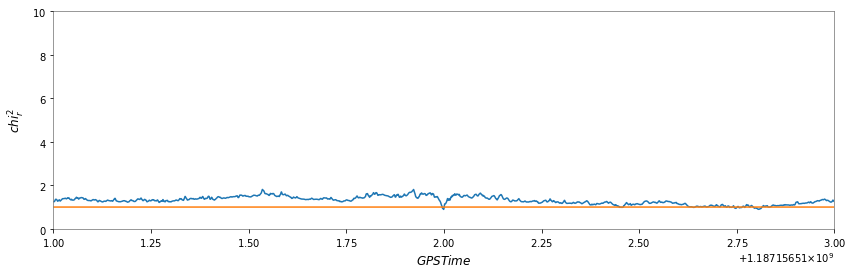
\includegraphics[width = .9\textwidth]{chi2 laplace b=2.png}
\caption{This figure shows the resulting $\chi^2_r$ statistic for perfectly Laplacian noise with $b=2$ scaled down by a factor of $10^{-21}$. The graph is zoomed in to show just the two-second time interview around the time of expected signal. A relatively weak dip toward unity is seen at time $t = 35.0$s.}
\centering
\end{figure} 

\begin{figure}[t]
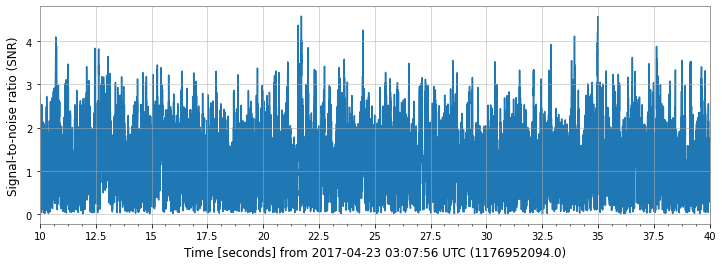
\includegraphics[width = .9\textwidth]{laplacian b=3 template 1.png}
\caption{This figure shows the resulting cropped SNR $\rho(t)$ after matched filtering was applied to recover the template signal from perfectly Laplacian noise with $b=3$, scaled down by a factor of $10^{-21}$. A signal peak was detected at time $t = 21.7$s with SNR $\rho = 4.6$.}
\centering
\end{figure}
\end{widetext}

\subsubsection{$\chi^2$-consistency testing and SNR re-weighting} \label{chisqaured}

As described in the previous section on matched filtering, the algorithm breaks down in the presence of spurious noise sources such as glitches and non-Gaussian and/or non-stationary noise. When this happens, matched filtering gives rise to elevated signal-to-noise peaks that are due to noise instead of gravitational waves of astrophysical origins, further complicating the detection data analysis pipeline. To address this issue, many existing detection pipelines, such as the PyCBC pipeline \cite{veto}, employ the use of signal consistency testing to distinguish between real signals and false ones due to noise. There are different methods to perform consistency testing on Virgo/LIGO data. In this paper, we make use of the $\chi^2$ time-frequency discriminator test described with great details in \textit{Allen (2005)} \cite{Allen_2005} and implemented in PyCBC's search pipelines \cite{pycbc}. The general purpose of the $\chi^2$ test is to see how much different ranges of frequencies of the template waveform contribute to the signal-to-noise ratio $\rho(t)$. The overall algorithm goes as follows. We first divide our template up into $p$ frequency sub-intervals (or\textit{ frequency bins}) $\Delta f_1,\Delta f_2,..., \Delta f_p$ with corresponding signal-to-noise ratios $\rho_1,\rho_2,...,\rho_p$. Then, we compute the extent to which a particular frequency bin contributes to $\rho(t)$ by calculating a $\chi^2$ test statistic as follows:
\begin{equation} 
    \chi^2 = \sum^p_{i=0}\left(\left|\rho_i - \frac{\rho}{p}\right|\right)^2
\end{equation}
where $\chi^2$ has a classical $\chi^2$ probability density distribution with degrees of freedom $\nu = 2(p-1)$ since the signal-to-noise ratio $\rho$ is a complex valued number. If the template matches closely with signal-to-noise output at a certain bin, the $\chi^2$ test statistic should be close to $\nu$. In this paper, we will be normalizing $\chi^2$ as follows 
\begin{equation}
    \chi^2_{r} = \frac{\chi^2}{\nu}
\end{equation}

The reduced chi-squared value $\chi^2_r$ would then approach unity when the template matches well with the signal-to-noise and deviate from that when it does not.

Using the reduced $\chi_r^2$ value, we can then `re-weigh' our signal-to-noise ratio $\rho(t)$ by utilizing the fact that $\chi_r^2$ describes the degree to which the SNR deviates from the template. The `re-weighted' SNR, denoted $\hat{\rho}$, is computed by scaling $\rho$ as follows:
\begin{equation}
    \hat{\rho} = \rho \,\cdot \,
    \begin{cases}
    1     & \quad\quad\text{if}\quad \chi^2_r\leq1\\
     \left[\frac{1}{2} + \frac{1}{2}(\chi^2_r)^3\right]^{-1/6}   & \quad\quad\text{if}\quad \chi^2_r>1
    \end{cases}
\end{equation}

Note that this process of re-weighing the SNR down-weighs $\rho$ where it is not strongly matched by the template used in the computation of $\rho$ and does the opposite where the template closely aligns with $\rho(t)$.

\begin{figure}[t]
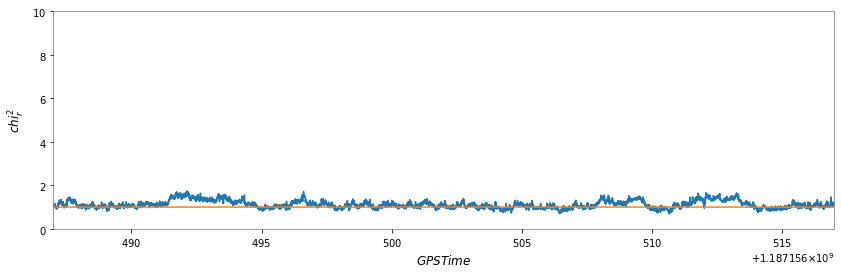
\includegraphics[width = .9\textwidth]{chi2 laplace b=3 zoomed.png}
\caption{This figure shows the resulting $\chi^2_r$ statistic for perfectly Laplacian noise with $b=3$ scaled down by a factor of $10^{-21}$. A very weak dip toward unity is seen at time $t = 35.0$s.}
\centering
\end{figure} 

\begin{figure}[t]
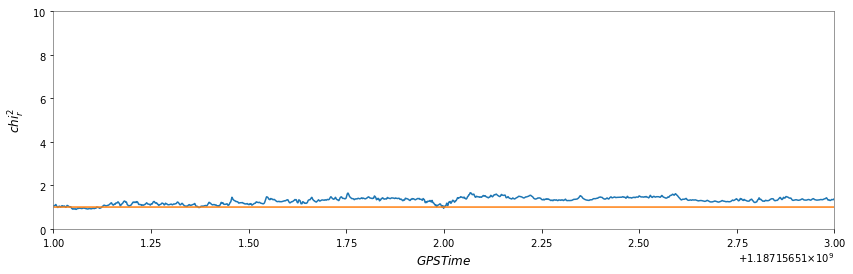
\includegraphics[width = .9\textwidth]{chi2 laplace b=3.png}
\caption{This figure shows the resulting $\chi^2_r$ statistic for perfectly Laplacian noise with $b=3$ scaled down by a factor of $10^{-21}$. The graph is zoomed in to show just the two-second time interview around the time of expected signal. A tiny dip toward unity is seen at time $t = 35.0$s.}
\centering
\end{figure} 

\begin{figure}[t]
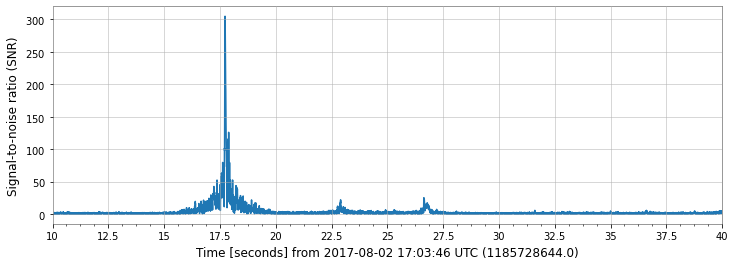
\includegraphics[width = .9\textwidth]{glitch loud 69 template 1.png}
\caption{This figure shows the resulting cropped SNR $\rho(t)$ after matched filtering was applied to recover the template signal from Glitch 1. A signal peak was detected at time $t = 17.7$s with SNR $\rho = 305.0$.}
\centering
\end{figure}

\begin{figure}[t]
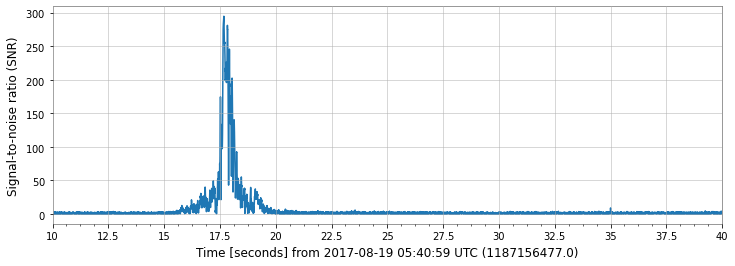
\includegraphics[width = .9\textwidth]{glitch loud 02 template 1.png}
\caption{This figure shows the resulting cropped SNR $\rho(t)$ after matched filtering was applied to recover the template signal from Glitch 2. A signal peak was detected at time $t = 17.7$s with SNR $\rho = 294.6$.}
\centering
\end{figure}

\section{Methodology} \label{method}

\begin{figure}[t]
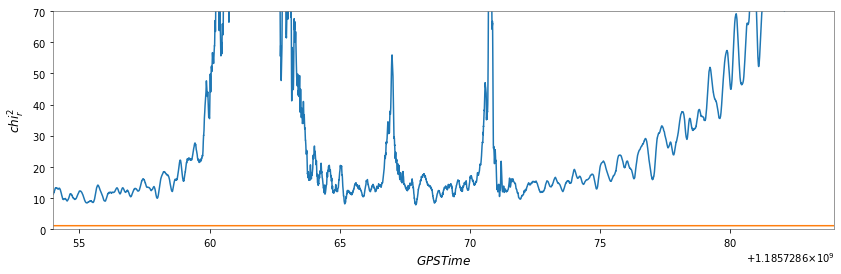
\includegraphics[width = .9\textwidth]{chi2 glitch 1 zoomed.png}
\caption{This figure shows the resulting $\chi^2_r$ statistic for Glitch 1. $\chi_r^2(t)$ is extremely large and fluctuates frequently with no apparent dip near the expected time $t=35$s.}
\centering
\end{figure} 

\begin{figure}[t]
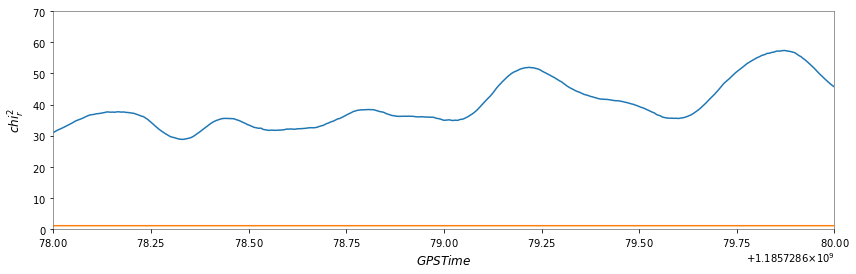
\includegraphics[width = .9\textwidth]{chi2 glitch 1.png}
\caption{This figure shows the resulting $\chi^2_r$ statistic for Glitch 1. The graph is zoomed in to show just the two-second time interview around the time of expected signal. $\chi_r^2(t)$ is extremely large and no apparent dip near the expected time $t=35$s was found.}
\centering
\end{figure} 

The following \textit{subsection A} discusses the methodology used in the performance evaluation of matched filtering and $\chi^2$-consistency testing in the presence of noise with known distributions as well as transient glitches. Then, in \textit{subsection B}, I provide the procedures undertaken in demonstrating the performance of matched filtering and $\chi^2$-consistency testing for a \textit{Blip} glitch found near event GW170814. All data analysis techniques (matched filtering and $\chi^2$-consistency testing) were implemented through the PyCBC software package \cite{pycbc}. All Python script implementation of this paper's methodology can be found at \footnote{V. Nguyen, Google Colab notebook for signal matched filtering and chi-squared consistency testing, \href{https://colab.research.google.com/drive/10q3SdhNjWyoZaVPdLqyoCEsSovplvMrK?authuser=2#scrollTo=7cafQoPiH5Sy}{(2020)}. URL: \url{https://colab.research.google.com/drive/10q3SdhNjWyoZaVPdLqyoCEsSovplvMrK?usp=sharing}}.

\subsection{Performance of matched filtering and $\chi^2$-consistency testing in different noise conditions}

\subsubsection{Performance in the presence of Gaussian and Laplacian noise} \label{gaussian}

In this paper, I considered two main types of noise distributions – Laplacian and Gaussian – with small variations in the Laplacian case, making the total number of noise distributions analyzed to be four. The analyzed noise distributions are as follows:
\begin{itemize}
    \item Perfectly Gaussian noise with $\mu = 0$  and $\sigma = 1$ scaled down by a factor of $10^{-21}$.
    \item Laplacian noise with location $\mu = 0$ and scale parameter $b = 1,2,3$. Laplacian noise with  $\mu = 0$ and varying $b$ was chosen for the purposes of this study due to its symmetric nature (similar to Gaussian noise) and varying levels of kurtosis. The higher the scale value $b$, the heavier the Laplacian noise distribution will be at the tails (note that heavier tails correspond to higher kurtoses). These Laplace distributed noise models were all scaled down by a factor of $10^{-21}$. An illustration of these distributions are shown in FIG. 3.
\end{itemize}

\begin{figure}[t]
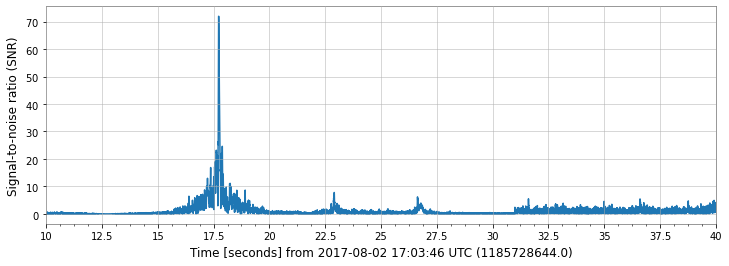
\includegraphics[width = .9\textwidth]{reweighted glitch 1.png}
\caption{This figure shows the resulting reweighted SNR $\hat{\rho}(t)$ using the computed $\chi^2_r$ statistic for Glitch 1.}
\centering
\end{figure} 

\begin{figure}
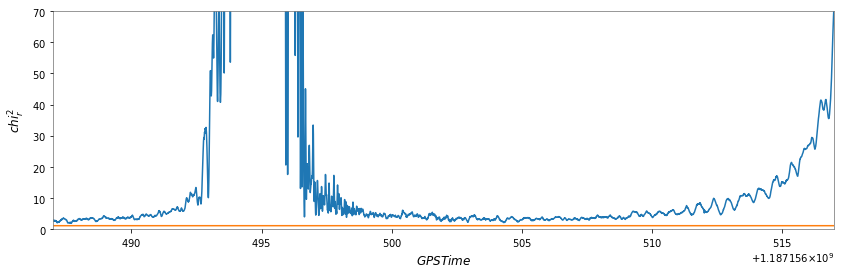
\includegraphics[width = .9\textwidth]{chi2 glitch 2 zoomed.png}
\caption{This figure shows the resulting $\chi^2_r$ statistic for Glitch 2 zoomed out to the entire search time interval.}
\centering
\end{figure}

Pure Gaussian noise was generated via the Python NumPy package's \code{random.normal} method then scaled down by a factor of $10^{-21}$ \cite{numpy}. As for the Laplacian noise, the \code{random.laplace} method was used. It was then scaled down accordingly similar to the Gaussian case. These noise stretches are all 50 seconds in length. Their sampling rate, and all subsequent time-series data described in this paper are $4096$ Hz – down-sampled from LIGO's original $16384$ Hz sampling rate.

\begin{widetext}
\begin{figure}[t]
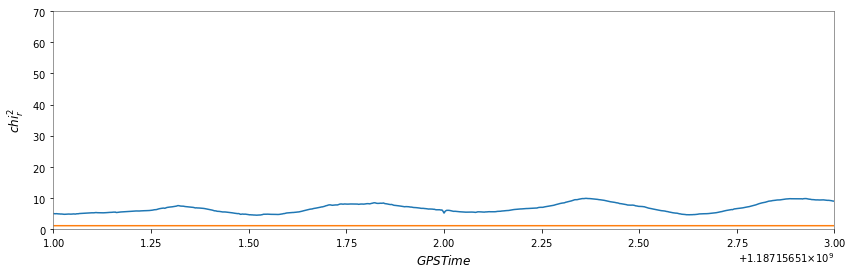
\includegraphics[width = .9\textwidth]{chi2 glitch 2.png}
\caption{This figure shows the resulting $\chi^2_r$ statistic for Glitch 2. The graph is zoomed in to show just the two-second time interview around the time of expected signal. $\chi_r^2(t)$ is moderately large with a very small dip toward unity at the expected time $t=35$s.}
\centering
\end{figure} 

\begin{figure}[t]
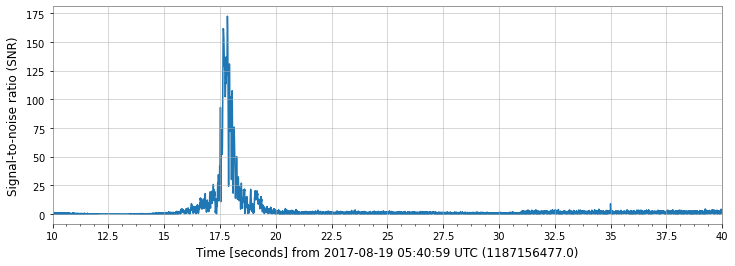
\includegraphics[width = .9\textwidth]{reweighted glitch 2.png}
\caption{This figure shows the resulting reweighted SNR $\hat{\rho}(t)$ using the computed $\chi^2_r$ statistic for Glitch 2. It can be seen that there is a moderately distinct $\hat{\rho}(t)$ peak at time $t=35$s with a value of $\hat{\rho}(t)=9.0$}
\centering
\end{figure}
\end{widetext}

\begin{figure}[t]\label{snr 3}
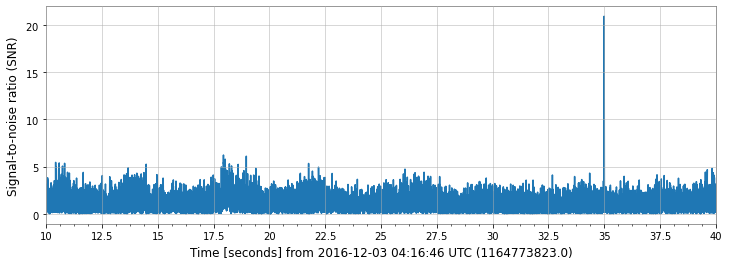
\includegraphics[width = .9\textwidth]{glitch 3 template 1.png}
\caption{This figure shows the resulting cropped SNR $\rho(t)$ after matched filtering was applied to recover the template signal from Glitch 3. A signal peak was detected at time $t = 35.0$s with SNR $\rho = 20.9$.}
\centering
\end{figure}

\begin{figure}[t]
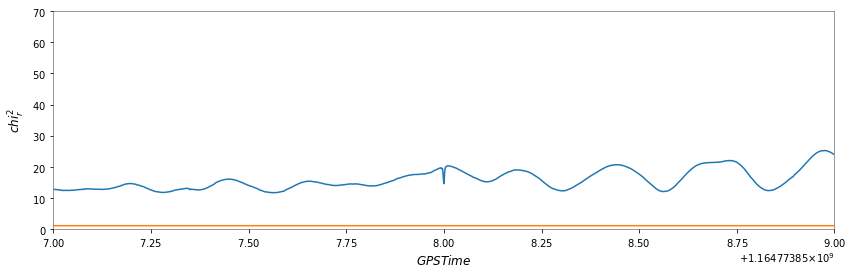
\includegraphics[width = .9\textwidth]{chi2 glitch 3.png}
\caption{This figure shows the resulting $\chi^2_r$ statistic for Glitch 3. The graph is zoomed in to show just the two-second time interview around the time of expected signal. There is a moderately strong dipc toward unity at the expected time $t=35$s.}
\centering
\end{figure} 

Then, I created a 50-second time-series template using post-Newtonian approximation theory (a method of approximating Einstein's field equations). The time-series template generation was done using PyCBC's \code{get\_td\_waveform} method; I also only used the plus polarization of the template waveform since this paper studies only the performance of signal extraction algorithms, not the waveforms themselves. The template waveform was of a binary black hole inspiral with masses 30 $M$\textsubscript{\(\odot\)} and 23 $M$\textsubscript{\(\odot\)} at an effective distance of 500 Mpc and initial frequency of 14 Hz. The waveform and was created using the `IMRPhenomD' model as the approximant. This template waveform in shown in FIG. 4.


I then proceeded to zero-pad the template so that its length matches the length of the 50-second stretch of noise. Afterwards, I `rolled' the templates so that they start at time $t=35$s in the 50-second stretch of data. A signal injection was then carried out to inject the template waveforms into the pure 50-second noise stretch. 

Afterwards, I estimated the PSD of the data. Then, I applied the PyCBC matched filtering algorithm using the \code{matched\_filter} method. The signal-to-noise ratio (SNR) $\rho (t)$ computed from the matched filtering algorithm was then cropped by 10 seconds on both ends. The reason for this is that applying the matched filter on a data segment of finite length using an estimated PSD gives rise to `edge effects'. In simplest terms, these `edge effects' give extremely high, false SNR peaks near the edges that can be mistaken for gravitational wave signal; thus, $\rho(t)$ needed to be trimmed on both ends. Then finally, I applied the $\chi^2$-consistency test using 40 frequency bins on this trimmed SNR $\rho(t)$ and proceeded to re-weigh it to find $\hat{\rho}(t)$ as described in \textit{subsection \ref{chisqaured}}. Using the cropped SNR $\rho(t)$ as well as the results of the $\chi^2$ test, I could then analyze them to evaluate the search's performance. 

\subsubsection{Performance in the presence of glitches}

The last aspect of this study is to evaluate the performance of matched filtering and $\chi^2$-consistency testing in the presence of transient glitches. In this paper, I used five samples of known Virgo/LIGO glitches with two \textit{`Extremely Loud'} glitches, one \textit{Scattered Light} glitch, one \textit{Whistle} glitch, and one \textit{Power Line} glitch. The glitch samples chosen for this study are as follows (note that the GPS times indicate times of greatest amplitude):

\begin{itemize}
\item Glitch 1: An \textit{`Extremely Loud'} glitch found at the Virgo detector on August 2$^{\text{nd}}$, 2017, 17:04:11 UTC (GPS time 1185728669).

\item Glitch 2: Another \textit{`Extremely Loud'} glitch, also found at the Virgo detector but on August 19$^{\text{nd}}$, 2017, 05:41:24 UTC (GPS time 1187156502).

\item Glitch 3: A \textit{Scattered Light} glitch found at the Livingston detector on December 3$^{\text{rd}}$, 2016, 04:17:11 UTC (GPS time 1164773848).

\item Glitch 4: A \textit{Power Line glitch} found at the Hanford detector on August 15$^{\text{th}}$, 2017, 01:59:25 UTC (GPS time 1186797583).

\item Glitch 5: A \textit{Whistle} glitch found at the Livingston detector on April 23, 2017, 03:08:21 UTC (GPS time 1176952119).
\end{itemize}

To extract and make use of these glitches,  I employed 25 seconds before and after their times of peak amplitude. Note that these samples of glitches also contain background noise that may or may not be Gaussian and stationary in addition to the glitches themselves. Removing background noise from these samples and extracting these glitches require complex methods that were not attainable within the time frame of the writing of this paper. A full catalog documentation of known Virgo/LIGO transient glitches from which these glitches were acquired was provided by Michael Zevin (PhD Candidate at Northwestern University) and the GravitySpy team. \cite{gravityspy}. 

For visualization purposes, strain time-series data of the glitches and their Q-transformed spectrograms are shown from FIG.\ 5.\ to FIG.\ 9.\ Note that the Q-transform is a special filter that mirrors the Fourier transform, often used to pick out special features of gravitational wave signals, highlighting signals with higher energy intensities. The mathematical details of this analysis technique can be found in \textit{Chatterji et.\ al (2004)} \cite{qtransform}.  With these 50 seconds long glitch segments in hand, I then proceeded to follow the same injection, recovery, and consistency testing procedures discussed in \textit{subsection \ref{gaussian}}. 

\begin{figure}[t]
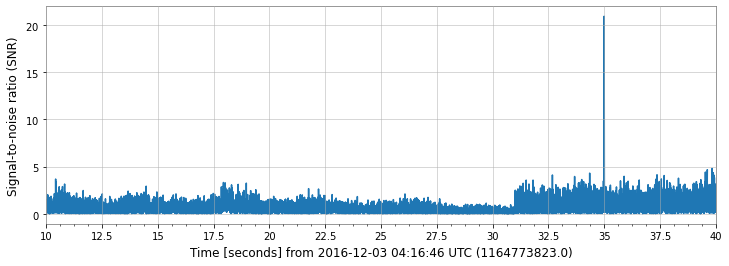
\includegraphics[width = .9\textwidth]{reweighted glitch 3.png}
\caption{This figure shows the resulting reweighted SNR $\hat{\rho}(t)$ using the computed $\chi^2_r$ statistic for Glitch 3. The peak re-weighted SNR remained the same as the previous case with $\hat{\rho}(t)=20.9$ at time $t=35.0$s.}
\centering
\end{figure}

\begin{figure}[t] \label{snr 4}
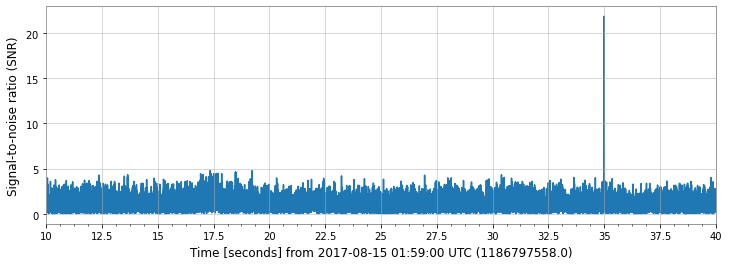
\includegraphics[width = .9\textwidth]{glitch 4 template 1.png}
\caption{This figure shows the resulting cropped SNR $\rho(t)$ after matched filtering was applied to recover the template signal from Glitch 4. A signal peak was detected at time $t = 35.0$s with SNR $\rho = 21.8$.}
\centering
\end{figure}

\subsection{Performance of matched filtering and $\chi^2$-consistency testing in distinguishing between event GW170814 and a nearby \textit{Blip} glitch found at the Livingston detector}

On August 14$^{\text{th}}$, 2017, 10:30 UTC, both LIGO detectors in Hanford and Livingston as well as the Virgo Observatory in Italy detected a binary black hole coalescence with initial masses 30.5 $M$\textsubscript{\(\odot\)} and 25.3 $M$\textsubscript{\(\odot\)}, called event GW170814 \cite{blip}. However, just about six seconds before the detection of GW170814 at the LIGO Livingston detector, a \textit{Blip} glitch occurred. Although this \textit{Blip} glitch was quiet and narrow enough so that it did not significantly affect the detection results of event GW170814, it still created a spurious SNR peak in the resulting $\rho(t)$ after matched filtering the data. To address this issue, $\chi^2$-consistency testing and SNR re-weighting were employed. In this paper, I sought to analyze the performance of matched filtering and $\chi^2$-consistency testing in distinguishing between event GW170814 and the \textit{Blip} glitch by analyzing the data and finding the signal myself, using a modified Python script referenced from GWOSC's 2020 Open Data Workshop, Tutorial 2.3 \cite{collaboration2019open}.

First, a 15-second data segment around event GW170814 that includes the blip glitch was queried directly from GWOSC. A visualization of this \textit{Blip} glitch can be found in FIG.\ 10. Then afterwards, matched filtering and $\chi^2$-consistency testing were applied in a similar fasion as described in the previous subsection. In this case, however, since the data segment is much shorter than the 50 seconds duration in the previous section, only 2 seconds of data on the edges were cropped. Using this calculated $\chi_r^2$ statistic, I then performed an SNR re-weighting to obtain $\hat{\rho}(t)$. With this information in hand, I could then evaluate the performance of matched filtering and the $\chi^2$-consistency test.



\section{Preliminary Results and Data Analysis} \label{results}

\subsection{Results for the case of Gaussian and Laplacian noise}
Since this template was zero-padded and rolled so that it starts at time $t=35$s referenced from the beginning of the noise/glitch data stretch before being injected, the peak-SNR after matched filtering is expected to be at time $t=35$s. The PyCBC matched filtering and $\chi^2$-consistency testing algorithms yielded reasonable results.

It can be seen from FIG.\ 11.\ and FIG.\ 14.\ for the perfect Gaussian noise and the Laplacian noise with $b=1$ cases that there are clear, thin, and distinct SNR peaks at time $t = 35.0$s. The peak SNR's of these two cases, though, are of different values. In the case of Gaussian noise, the SNR is 20.0, while it is only 12.6 in the case of Laplacian noise with $b=1$. Furthermore, it can also be seen that the SNR `noise-floor' in FIG.\ 11.\ is similar to that in FIG.\ 14. Specifically in both cases, the SNR `noise-floor' varies around $\rho = 3.75$. Looking at the $\chi^2_r$ results for these two cases in FIG. 12.\ and 13.\ (Gaussian noise) and FIG. 15.\ and 16.\ (Laplacian with $b=1$ noise), we can also see some similarities. The $\chi^2_r$ graphs for both cases show a strong dip at the expected time $t=35$s, indicating a strong correlation between high SNR and template contribution. It is also worthy to note that in both of these cases, the $\chi^2_r$ value grows just around the strong dip. The reason for this is because at these times around $t=35$s, the template contributes to the high SNR but does not perfectly align with it \cite{collaboration2019open}. In the Gaussian case, however, the $\chi_r^2$ value climbs to a higher value compared to the Laplacian with $b=1$ case around the expected time (reaching a maximum of $\chi_r^2 \approx 7$ for the Gaussian case and $\chi_r^2\approx 4$ for the Laplacian case with $b=1$). This is also expected since high $\chi_r^2$ values just around a strong dip toward unity indicates that the background noise fits the Gaussian model well.

\begin{figure}
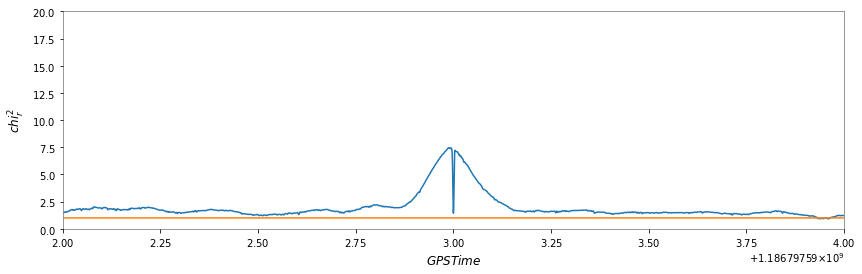
\includegraphics[width = .9\textwidth]{chi2 glitch 4.png}
\caption{This figure shows the resulting $\chi^2_r$ statistic for Glitch 4. The graph is zoomed in to show just the two-second time interview around the time of expected signal. There is a moderately strong dip toward unity at the expected time $t=35$s.}
\centering
\end{figure} 

\begin{figure}[t]
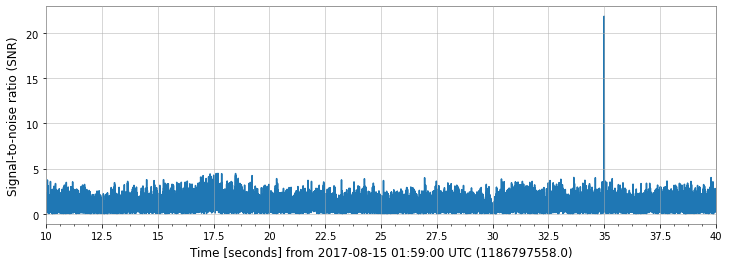
\includegraphics[width = .9\textwidth]{reweighted glitch 4.png}
\caption{This figure shows the resulting re-weighted SNR $\hat{\rho}(t)$ using the computed $\chi^2_r$ statistic for Glitch 4. The peak re-weighted SNR remained the same as the previous case with $\hat{\rho}(t)=21.8$ at time $t=35.0$s.}
\centering
\end{figure}

In the case of Laplacian noise with $b=2$ (FIG.\ 17.), the detection result was also accurate (i.e.\ there is a clear, thin, and distinct peak at time $t=35.0$). However, in this case, the SNR $\rho(t)$ is much lower, reaching only a value of $6.1$. Furthermore, it can be seen that the SNR `noise floor' is also relatively consistent with the Gaussian noise case and the $b=1$ Laplacian noise case, fluctuating around $\rho = 3.0$, though many times reaching $\rho = 4.0$. Looking at FIG. 18.\ and FIG. 19.\ for the $\chi_r^2$ graphs, however, it can be seen that there are distinct differences compared to the Gaussian case or the Laplacian case with $b=1$. In this Laplacian case with $b=2$, the dip toward unity at time $t=35$s is much weaker as $\chi^2_r$ in the region around it does not climb as high, indicating that the noise background is getting less and less Gaussian as expected. 

In the case of Laplacian noise with scale parameter $b=3$, however, we can make new interesting observations. As shown in FIG.\ 20., the SNR function $\rho(t)$ has no clear and distinct peaks. Throughout the entire time interval, $\rho(t)$ appears to fluctuate randomly around $\rho = 3$. The function's highest SNR is 4.6, located at time $t=21.7$s, which is clearly inaccurate. However, it is still noteworthy that the SNR value at time $t=35$s is still higher than its surroundings, coming close to the maximum value found at time $t=21.7$s. Looking at FIG.\ 21.\ and FIG.\ 22.\ for the $\chi_r^2$ statistic, we can see that there is a very small dip toward unity at the expected time $t=35$s, indicating that there exists a very weak signal at that time. Note that this dip is a lot weaker compared to the cases of Gaussian noise and Laplacian noise with $b=1,2$ – where the dip is much more apparent even when zoomed out to the entire time interval.


Note that in all the four cases presented above (Gaussian noise, Laplacian noise with $b=1$, $b=2$, $b=3$), the reweighted SNR's $\hat{\rho}(t)$ are extremely similar if not identical with $\rho(t)$. In the first three cases – Gaussian, Laplacian with $b=1$, and Laplacian $b=2$ – the explanation is that all of these these three situations already have clear and distinct peaks with close-Gaussian (Laplacian with $b=1$) or perfect Gaussian noise itself. Therefore, the re-weighing function had little effects. In the last case (Laplacian with $b=3$), the re-weighting function had little effects not because the noise is Gaussian or close-Gaussian; rather, it was because the noise was \textit{too loud}, rendering the matched filter's ability to pick the signal out of the noise. Note that the $\chi^2$-cosistency test only re-weighs $\rho(t)$ so that the \textit{detected} signal from matched filtering is amplified, not to dig out signal from louder noise as an \textit{alternative} to matched filtering itself. For this reason, $\hat{\rho}(t)$ graphs for these cases were omitted from this paper.

\begin{widetext}

\begin{figure}[t]
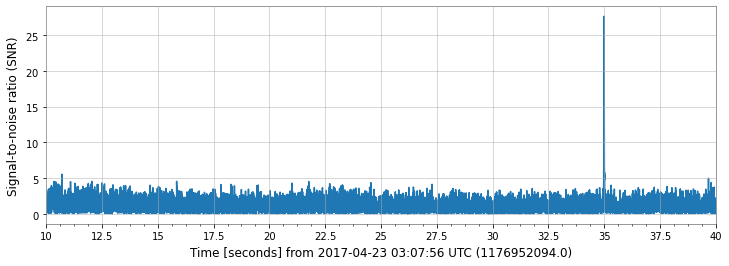
\includegraphics[width = .9\textwidth]{glitch 5 template 1.png}
\caption{This figure shows the resulting cropped SNR $\rho(t)$ after matched filtering was applied to recover the template signal from Glitch 5. A signal peak was detected at time $t = 35.0$s with SNR $\rho = 20.9$.}
\centering
\end{figure}

\begin{figure}
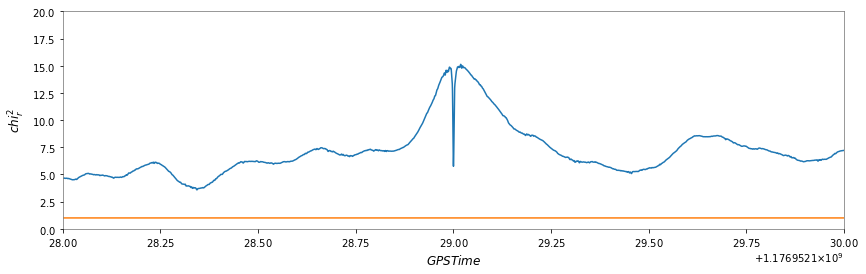
\includegraphics[width = .9\textwidth]{chi2 glitch 5.png}
\caption{This figure shows the resulting $\chi^2_r$ statistic for Glitch 5. The graph is zoomed in to show just the two-second time interview around the time of expected signal. There is a rather strong dip toward unity at the expected time $t=35$s.}
\centering
\end{figure} 

\end{widetext}


\subsection{Results for the case of transient glitches}

\begin{figure}[t]
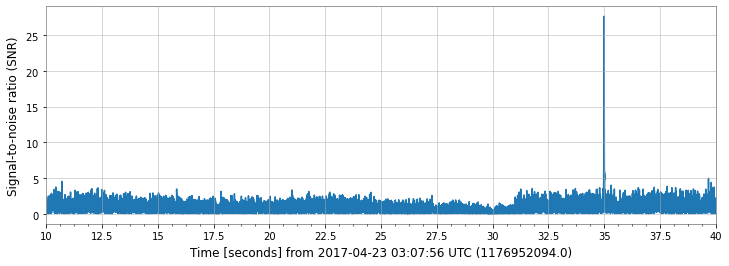
\includegraphics[width = .9\textwidth]{reweighted glitch 5.png}
\caption{This figure shows the resulting re-weighted SNR $\hat{\rho}(t)$ using the computed $\chi^2_r$ statistic for Glitch 5. The peak re-weighted SNR remained the same as the previous case with $\hat{\rho}(t)=27.6$ at time $t=35.0$s.}
\centering
\end{figure}

Figures 23.\ and 24.\ show the detection results for the two \textit{Extremely Loud} glitches (Glitch 1 and Glitch 2). Both of these results share one thing common: They both have an extremely high SNR peak, ranging in the hundreds ($\rho=305.0$ and $\rho=294.6$). It is also worth noticing that these peaks are more triangular / pyramidal in shape – that is, the elevated SNR effects caused by \textit{Extremely Loud} glitches are spread out across multiple frequency bins, and subsequently heavily affect the time-domain data. Moreover, note that in FIG.\ 23., we can see that Glitch 1 also gave rise to several lower amplitude false-alarm SNR peaks in addition the highest peak found at time $t=17.7$s. Similar to the highest peaks, these peaks are more triangular in nature and are of unusually high amplitudes; thus, they can easily be differentiated from real gravitational wave signal. 

Considering the $\chi^2_r$ graphs for Glitch 1 in FIG.\ 25 and 26, we can see that the $\chi^2_r$ statistic is extremely high and contains no apparent dips at the expected time $t=35$s. This means that the buried signal would likely be missed in a real gravitational wave search if data analysis stopped here. However, considering the re-weighted SNR $\hat{\rho}(t)$ graph in FIG.\ 27., there is a small, but still relatively distinct peak at the expected time $t=35$s. It is also noteworthy to point out that the extremely high signal-to-noise amplitudes caused by the glitch was substantially reduced down to less than 80 from the initial maximum value of 294.6.  FIG. 28.\ and 29.\ shows the  $\chi^2_r$ graphs for Glitch 2. FIG.\ 30.\ shows the re-weighted SNR $\hat{\rho}(t)$ for Glitch 2. The results for Glitch 2 are similar to those of Glitch 1; they both have weak dips toward at the expected time $t=35$s for the $\chi_r^2$ statistic and damped-down glitches SNR after the re-weighting. However, it can be seen that there is a small but relatively distinct peak (more distinct compared to that of Glitch 1) at time $t=35$s, reaching a value of $\hat{\rho}(t)=9.0$ – indicating that a signal is likely to exist at this time for the case of Glitch 2.

Figures 31, 34, and 37 show the SNR results for the recovery of the template signal injected into Glitch 3, 4, and 5, respectively. Notice that all three of these cases resulted in similar peak SNRs, with all three results reaching a signal-to-noise ratio $\rho$ of around $20$. In addition to that, the SNR `noise floor' is similar all across of three cases, fluctuating at around $\rho\approx 4$. Furthermore, considering their $\chi_r^2$ statistic graphs (shown if FIG.\ 32, FIG.\ 35, and FIG.\ 38 for Glitch 3,4,5 respectively) we can see that three of these cases have rather strong and distinct dips toward unity at the expected time $t=35$s with the dip of Glitch 3 being slightly weaker than those of the other two. Note that Glitch 3 is rather spread out on the search-time interval, with concentrated noise power evenly distributed throughout; therefore, the result resulting weaker $\chi_r^2$ dip for Glitch 3 was reasonably expected. Similar to the case of Gaussian and Laplacian noise with $b=1$ and $b=2$, the re-weighting process had very little impact on the detection results for Glitch 3,4, and 5. The re-weighted SNR graphs for Glitch 3,4 and 5 are shown in FIG.\ 33, FIG.\ 36, and FIG.\ 39 respectively. The reason for this is also similar to the known noise distributions case – the original $\rho(t)$ already has a clear and distinct SNR peak and therefore consistency testing had little impact. However, it is worth to point out that the `noise background' in these cases were suppressed by consistency testing, thereby validating our original detection results.  

\subsection{Results for event GW170814 and the LIGO Livingston \textit{Blip} glitch}

\begin{figure}
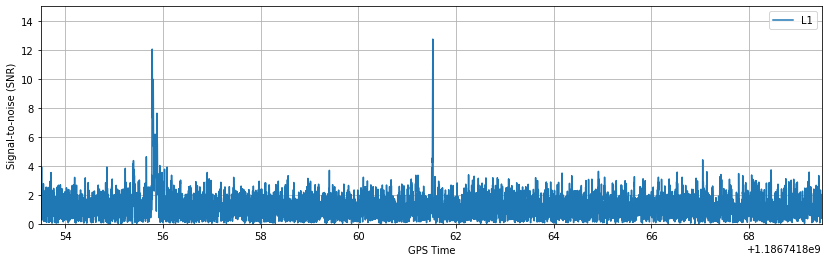
\includegraphics[width = .9\textwidth]{blip orig snr.png}
\caption{This figure shows the resulting SNR $\rho(t)$ event GW170814 and the nearby \textit{Blip} glitch. The first SNR peak is due to the glitch; it has a value of $\rho\approx12.0$. The second SNR peak is event GW170814; it has a value of $\rho\approx12.9$.}
\centering
\end{figure} 

\begin{figure}[t]
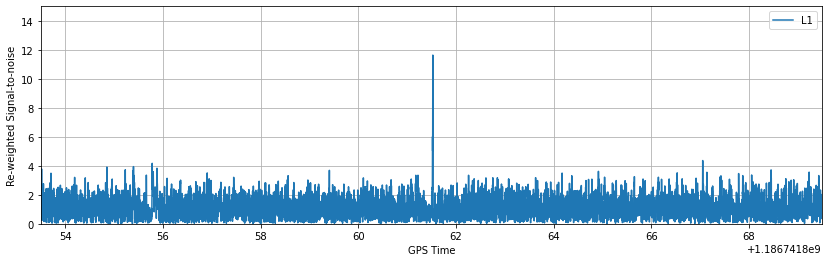
\includegraphics[width = .9\textwidth]{blip reweighted.png}
\caption{This figure shows the resulting re-weighted SNR $\hat{\rho}(t)$ using the computed $\chi^2_r$ statistic for event GW170814 and the nearby \textit{Blip} glitch. It can be seen that the initial peak due to the glitch in $\rho(t)$ has `disappeared'.}
\centering
\end{figure}

Figure 40 shows the resulting SNR $\rho(t)$ after matched filtering data from event GW170814 and the nearby \textit{Blip} glitch found at the LIGO Livingston detector. It can clearly be seen from this figure that there are \textit{two} thin and distinct signal-to-noise peaks with the first one having a value of $\rho\approx 12.0$ and the second one having a value of $\rho\approx 12.9$. According to the observation paper of event GW170814 published by the LIGO Collaboration in \cite{blip}, only the second peak represents the actual binary black hole coalescence. Without this knowledge beforehand, however, it is hard to distinguish between the two peaks to see which one actually comes from an astrophysical source. Therefore, computation of $\chi_r^2$ and SNR re-weighting is extremely crucial. Figure 41 shows the resulting re-weighted SNR $\hat{\rho}(t)$ using the computed $\chi_r^2$ statistic from the $\chi^2$-consistency test. In this figure, it can be seen that the first spurious SNR peak due to the glitch was completely suppressed, leaving only the real SNR-peak of the binary black hole coalescence to be found. 

\section{Conclusions} \label{conclusions}
From the results presented in \textit{subsection IV A}, it can be concluded that matched filtering performs best in stationary and perfect Gaussian noise. Furthermore, there is a strong positive correlation between the kurtosis of the Virgo/LIGO noise distributions and the performance of matched filtering. This observation agrees with the mathematical framework of the matched filtering detection algorithm. Although both Laplacian noise (regardless of scale parameter $b$) and Gaussian noise are symmetric about the y-axis, Laplacian noise distributions are much more tail-heavy. This means that when random noise was generated, louder noise was favored. Therefore, it makes mathematical sense that such a probability density distribution would induce a negative effect on the matched filtering detection algorithm. Furthermore, it can also be concluded that matched filtering in the presence of background noise with consistent probability distributions benefits little from the $\chi^2$-consistency test. In these cases, the $\chi^2$-consistency test either re-iterates the findings of matched filtering, or fail to identify a signal if matched filtering has previously failed.


From the results and data analysis discussed in \textit{subsection IV B} and \textit{IV C} , we can conclude that short-duration \textit{Extremely Loud} glitches have the greatest impact on the performance of matched filtering in gravitational wave detection. Specifically, \textit{Extremely Loud} glitches elevate the signal-to-noise ratio to unusually high levels and can easily mask out real gravitational wave signal. However, the effects of these glitches have distinct characteristics that are worth noting. First, these glitches elevate the signal-to-noise ratio to the extremes, reaching up to the hundreds in magnitude. This characteristic is in clear contrast with real gravitational wave signals, where the resulting SNRs are usually only 2 digits in magnitude. Second, elevated time-series SNR $\rho(t)$ peaks due to \textit{Extremely Loud} glitches have wide bottoms, looking almost pyramidal / triangular like over large time intervals. This is also starkly different from the characteristics of real gravitational wave signals, where the SNR peaks are thin and distinct with no wide bottoms, spanning only very small time intervals. Moreover, for signal detection accompanied with \textit{Extremely Loud} glitches, the use of $\chi^2$-consistency testing and SNR re-weighting is very important. Although the test does not perform as well if the glitches are exceedingly loud as in the case of Glitch 1, it still proves to be useful in picking out real signal in quieter glitches as in the case of Glitch 2.

In the cases of \textit{Scattered Light}, \textit{Power Line}, and \textit{Whistle} glitches, the noise background are generally low enough for matched filtering to detect  real signal from medium mass binary inspirals at an effective distance of $500$MPc. Therefore, since matched filtering already gives clear and distinct SNR peaks in these situations, the use of $\chi^2$-consistency testing and SNR re-weighting was not necessary; however, it was shown in the previous section (\textit{section IV}), that $\chi^2$-consistency testing does indeed increase the confidence in the detection results of matched filtering. From the results in \textit{subsection IV C}, it can be concluded that for relatively loud \textit{Blip} glitches that occur near a real signal of astrophysical origin, the use of $\chi^2$-consistency testing and SNR re-weighting is crucial in order to distinguish the real signal from the transient glitches.

In practice, real Virgo/LIGO data analysis procedures already have $\chi^2$-consistency testing and SNR re-weighting incorporated into their procedures where there are `data veto' guidelines based of the computed $\chi^2$ statistic. It has been shown in this paper that such techniques are essential in detecting real gravitational waves from astrophysical sources as in event GW170814. With this being said, however, the challenge lies in picking out real gravitational wave signals when they coincide with transient glitches; an example of this would be event GW170817 at the LIGO Livingston detector where a glitch coincided with the signal. In these cases, ordinary $\chi^2$-consistency testing and SNR re-weighting procedures presented in this paper are not sufficient. Therefore, future research should focus on developing comprehensive mathematical characterization of different classifications of non-Gaussian and transient glitches so that signals can be picked out from such noise backgrounds. Furthermore, considering that this paper has qualitatively demonstrated that there is relationship between the glitch's amplitude to the performance of $\chi^2$-consistency testing, further research could look for a quantitative relationship between these two values.

\section{Summary} \label{summary}
As mentioned, the detection of gravitational waves is especially challenging and requires extreme precision as well as sophisticated data analysis tools. In this paper, I presented two of the most common and efficient data analysis methods for the detection of gravitational waves – namely, matched filtering and $\chi^2$-consistency testing. I then proceeded to evaluate the performance of these two data analysis tools in different noise conditions while using event GW170814 as an illustrative example. Four consistent noise distributions and 6 different glitches were analyzed. Specifically, I considered Guassian noise, Laplacian noise with $b=1$, Laplacian noise with $b=2$, and Laplacian noise with $b=3$. As for the glitches, I employed 2 \textit{Extremely Loud} glitches, 1 \textit{Scattered Light} glitch, one \textit{Power Line} glitch, one \textit{Whistle} glitch, and one \textit{Blip} glitch (with the \textit{Blip} glitch being found near event GW170814).

Upon evaluation, I found that matched filtering performs best when detector noise is perfectly Gaussian and stationary. Matched filtering also performs considerably well when the noise distribution is close-Gaussian, namely Laplacian with $b=1$ and $b=2$. It was also shown that matched filtering breaks down when noise distributions are tail-heavy (that is, when they have high kurtoses such as the Laplacian with $b=3$ case). Furthermore, it was found that the existence of Extremely Loud glitches causes exceptionally high SNRs that can easily mask out true gravitational wave signals if the glitch and the signal coincide. In contrast, \textit{Scattered Light}, \textit{Power Line}, and \textit{Whistle} glitches are generally not loud enough to mask out true gravitational wave signals; \textit{Blip} glitches, however, can mimic real gravitational wave signals if they don't coincide. Moreover, I found that $\chi^2$-consistency testing has little impact in cases where matched filtering already has favorable results. In such situations, $\chi^2$-consistency testing only improves the confidence of the matched filtering detection. However, in the cases of \textit{Extremely Loud} and \textit{Blip} glitches, where matched filtering does not give accurate results on its own, the use of $\chi^2$-consistency testing is crucial in being able to pick out true gravitational wave signals. 

\begin{acknowledgments}
I would like to express my sincerest gratitude to Dr.\ Eric Myers at the State University of New York, New Paltz for guiding me at every step of the way in the making of this paper. Dr. Myers has guided me through my research from the very start, from teaching me the basic background knowledge to helping me with the writing process. I could not be more grateful of Dr.\ Myers' mentorship.

I would also like to thank Michael Zevin (PhD Candidate at Northwestern University), Dr.\ Peter Shawhan at the University of Maryland, and other scientists at the LIGO Scientific Collaboration (LSC), as well as the GravitySpy team for answering many of my technical questions and providing me with the data and documentation that without which, this research would not have been possible. 

This research has made use of data obtained from the Gravitational Wave Open Science Center (\url{https://www.gw-openscience.org}), a service of LIGO Laboratory, the LIGO Scientific Collaboration and the Virgo Collaboration. LIGO is funded by the U.S. National Science Foundation. Virgo is funded by the French Centre National de Recherche Scientifique (CNRS), the Italian Istituto Nazionale della Fisica Nucleare (INFN) and the Dutch Nikhef, with contributions by Polish and Hungarian institutes.
\end{acknowledgments}



\bibliography{citations.bib}% Produces the bibliography via BibTeX.

\end{document}
